\section{Mô tả design pattern và Deploy hệ thống}
\subsection{Kiến trúc các design pattern được sử dụng}
\indent Sau quá trình nghiên cứu và phát triển phần mềm cho hệ thống YoloFarm, nhóm đã áp dụng các Design Pattern (mẫu thiết kế) sau đây để đảm bảo kiến trúc rõ ràng, dễ bảo trì và dễ mở rộng:
\setlist[enumerate]{leftmargin=*,topsep=0pt,itemsep=2pt,parsep=0pt}
\setlist[itemize]{leftmargin=*,topsep=0pt,itemsep=2pt,parsep=0pt}
\begin{longtable}{|P{4.8cm}|m{10cm}|}\hline
    \hline
    \textbf{Design Pattern} & \centering\arraybackslash\textbf{Chi tiết áp dụng trong dự án} \\
    \hline

    \textbf{MVC (Model - View - Controller)} & Thư mục \texttt{server/src/models/} chứa các class/đối tượng định nghĩa cách tương tác với bảng trong cơ sở dữ liệu MySQL (Model). Thư mục \texttt{server/src/controllers/} chịu trách nhiệm nhận request từ người dùng, gọi các logic để xử lý dữ liệu và trả về kết quả (Controller). Phía Frontend ứng dụng React trong thư mục \texttt{client/src/pages/} và \texttt{components/} hiển thị dữ liệu lên màn hình (View). \\
    \hline
    \textbf{Middleware Pattern} & Áp dụng trong xây dựng API của Express.js nằm tại thư mục \texttt{server/src/middleware/}. Các request từ Client trước khi chuyển đến Controller sẽ đi qua các Middleware chặn lại để thực hiện: xác thực người dùng (Authentication qua JWT), kiểm tra tính hợp lệ dữ liệu và phân quyền hệ thống (Authorization). \\
    \hline
    \textbf{Observer / Pub-Sub Pattern} & Nhằm thiết lập truyền tải nhận dữ liệu thời gian thực. Bằng cách sử dụng giao thức MQTT kết nối với máy chủ Adafruit IO, server đóng vai trò chuyển tiếp như một "Publisher" và "Subscriber" lắng nghe dữ liệu liên tục do phần cứng gửi tới. Ngoài ra, Socket.IO cũng sử dụng Pub-Sub để đẩy tự động (push) các cảnh báo thông báo trực tiếp lên giao diện Frontend. \\
    \hline
    \textbf{Singleton Pattern} & Đảm bảo chỉ khởi tạo một thể hiện (instance) duy nhất của đối tượng trong toàn hệ thống. Ví dụ: instance kết nối cơ sở dữ liệu ở \texttt{server/src/config/db.js} hoặc module MQTT Node-Client luôn chỉ tồn tại một bản sao xuyên suốt ứng dụng. Với React Frontend, sử dụng React Context (như \texttt{AuthContext}, \texttt{ThemeContext}) qua Provider cũng là ứng dụng tương đương của Singleton để cung cấp trạng thái toàn cục (global state) cho ứng dụng. \\\hline
\end{longtable}
\subsection{Deploy hệ thống}
\indent Việc triển khai của YoloFarm được tổ chức theo đúng cấu trúc repo hiện tại: phần giao diện nằm ở \texttt{client/}, backend Node.js nằm ở \texttt{server/}, còn dịch vụ AI chạy tách biệt như một FastAPI space/container riêng. Trong giai đoạn phát triển, nhóm ưu tiên chạy local bằng \texttt{pnpm dev} để đồng bộ frontend, backend và AI service; khi đưa lên môi trường triển khai, các thành phần được đóng gói theo Docker Compose hoặc các nền tảng hosting tương ứng để giữ cấu hình nhất quán giữa máy lập trình và môi trường chạy thực tế.

\begin{figure}[H]
	\centering
	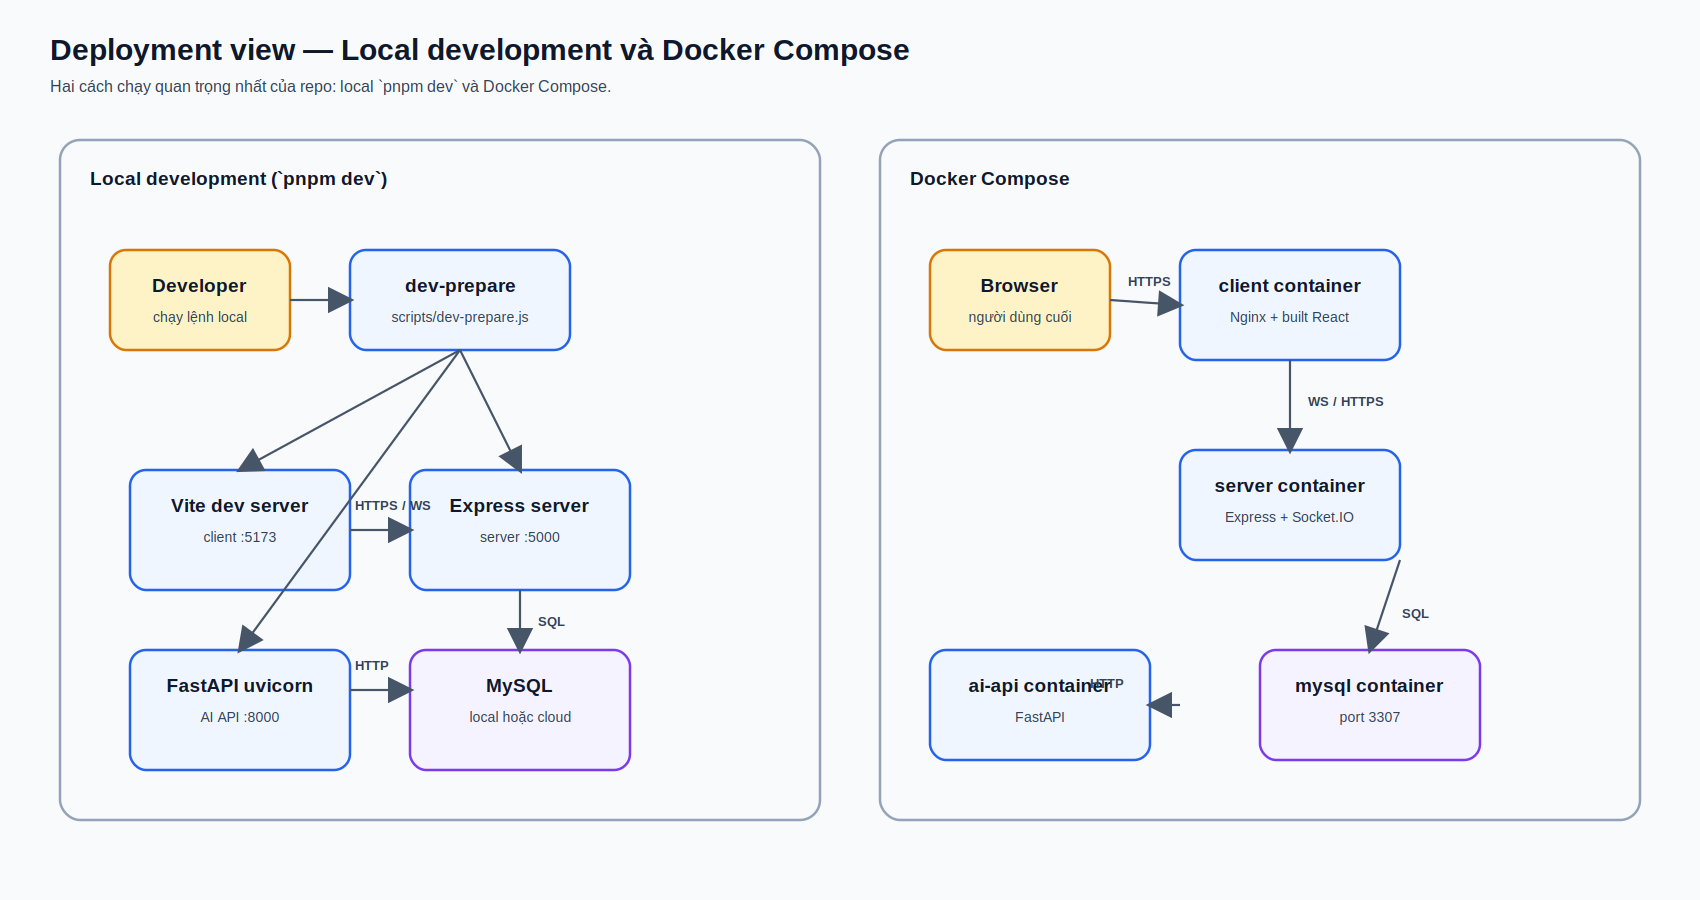
\includegraphics[width=0.92\linewidth]{./Pictures/Task_6/architecture/deployment-view.png}
	\caption{Sơ đồ triển khai của YoloFarm theo hai chế độ chạy local và Docker Compose}
\end{figure}

\subsubsection{Deploy frontend}
\indent Giao diện frontend của YoloFarm được triển khai trên \textbf{Vercel}. Mã nguồn được quản lý tại kho GitHub \texttt{yolofarm---group-6---L05---HK252}, từ đó Vercel tự động đồng bộ và kích hoạt quy trình CI/CD cho nhánh triển khai.

\indent Trên Vercel, các biến môi trường (Environment Variables) được cấu hình để frontend gọi đúng backend đang chạy trên Hugging Face Spaces, cụ thể là biến \texttt{VITE\_API\_URL} trỏ đến \url{https://cong2005-smartfarm-ai.hf.space/api}. Nhờ đó, người dùng có thể truy cập giao diện YoloFarm qua đường dẫn công khai: \url{https://smart-farmsmart-life.vercel.app/}.

\begin{figure}[H]
	\centering
	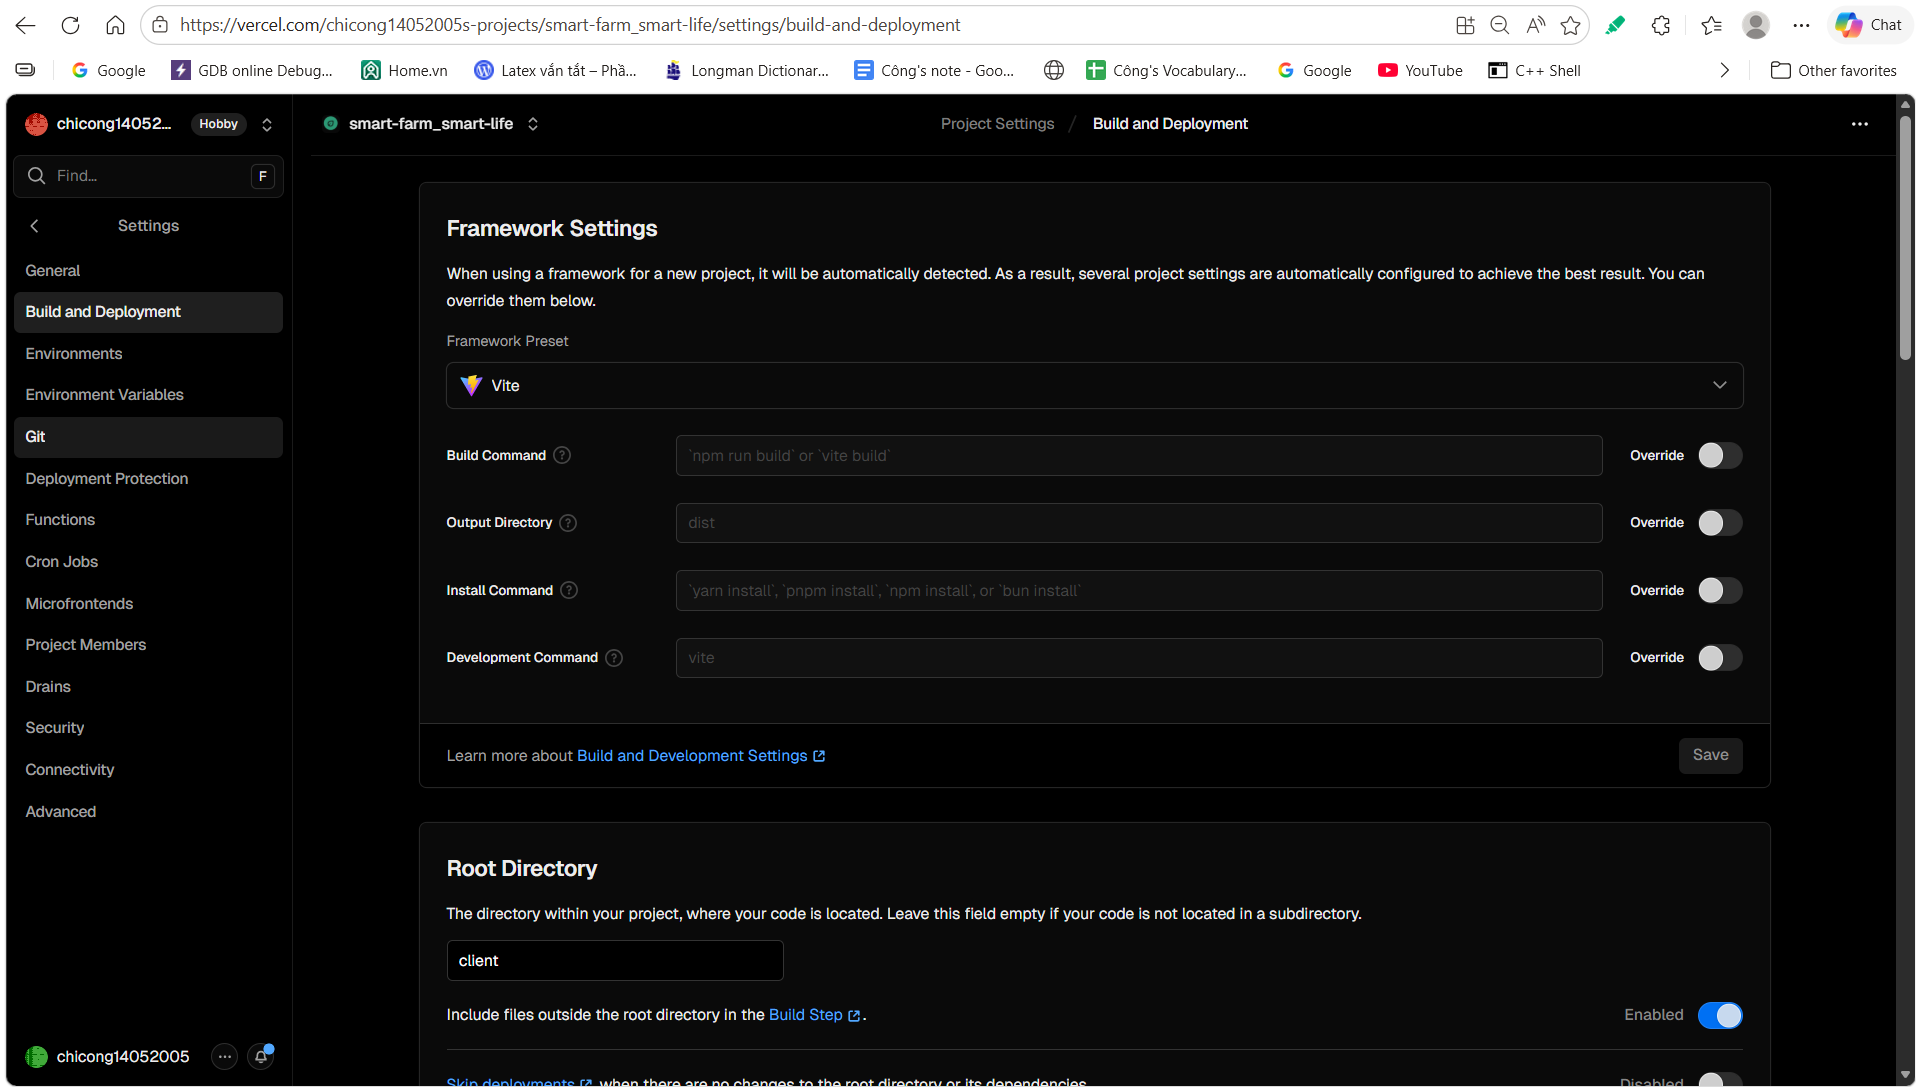
\includegraphics[width=0.8\linewidth]{./Pictures/Task_6/frontend_vercel.png}
	\caption{Giao diện Deployment phần mã nguồn Frontend trên Vercel}
\end{figure}
\subsubsection{Deploy backend}
\subsubsubsection{Phần server}
\indent Backend server của YoloFarm được triển khai trên \textbf{Hugging Face Spaces}. Thành phần Node.js được đóng gói bằng \texttt{Dockerfile} để giữ nguyên hành vi giữa môi trường local và môi trường chạy thật, đồng thời tách biệt rõ phần server với phần giao diện. Các lệnh khởi động và biến môi trường được khai báo ngay trong cấu hình container, giúp server có thể kết nối ổn định tới dịch vụ AI thông qua biến \texttt{AI\_API\_URL}.

\begin{figure}[H]
	\centering
	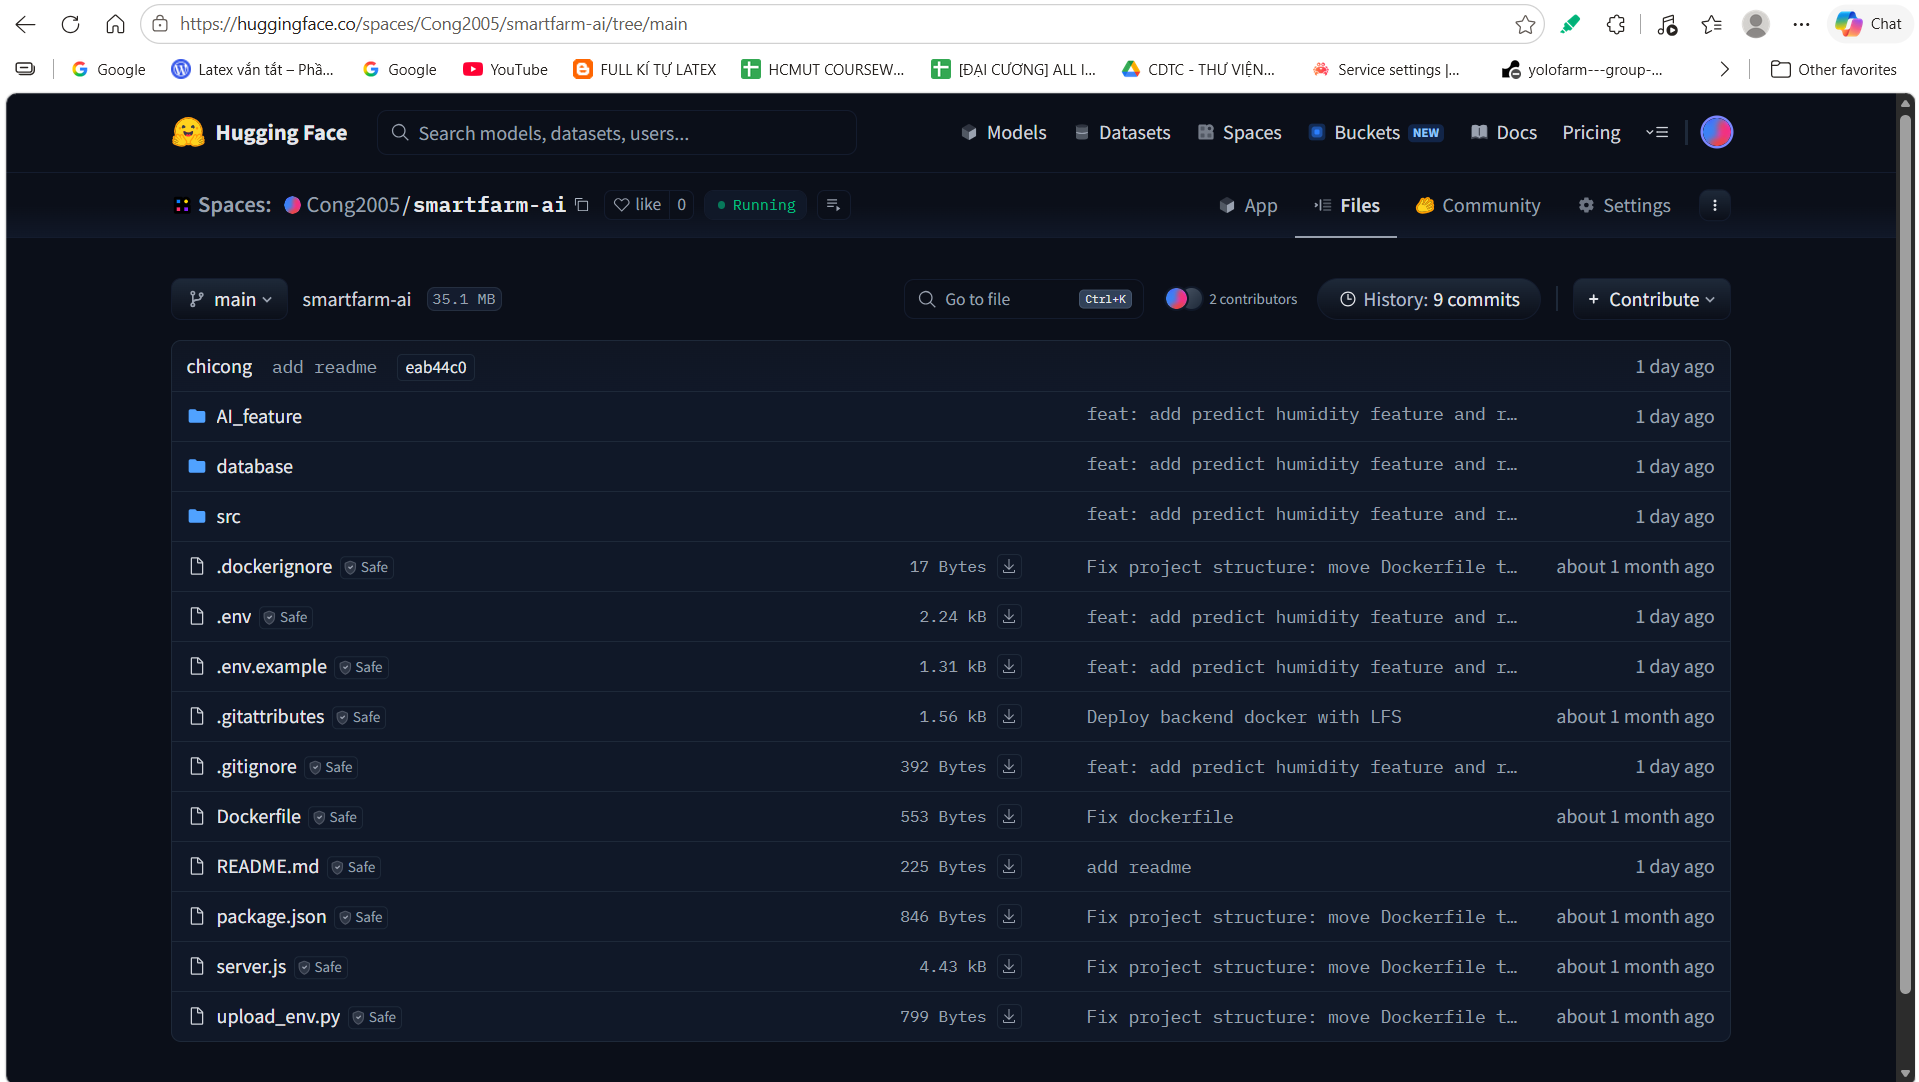
\includegraphics[width=0.8\linewidth]{./Pictures/Task_6/backend_server_files.png}
	\caption{Danh sách mã nguồn Backend Server chạy trên Hugging Face Spaces}
\end{figure}

\subsubsubsection{Phần các tính năng AI}
\indent Dịch vụ AI của YoloFarm được vận hành như một \textit{Space độc lập} để tối ưu tài nguyên cho suy luận mô hình. Space này tự cài các thư viện Python được khai báo trong \texttt{requirements.txt} và sử dụng mô hình đã huấn luyện tại tệp \url{https://huggingface.co/spaces/Cong2005/SmartFarm_api/blob/main/pest_detection/api/plant_disease_recog_model_pwp_5.keras} để phân loại bệnh lá cây từ ảnh đầu vào.

\begin{figure}[H]
	\centering
	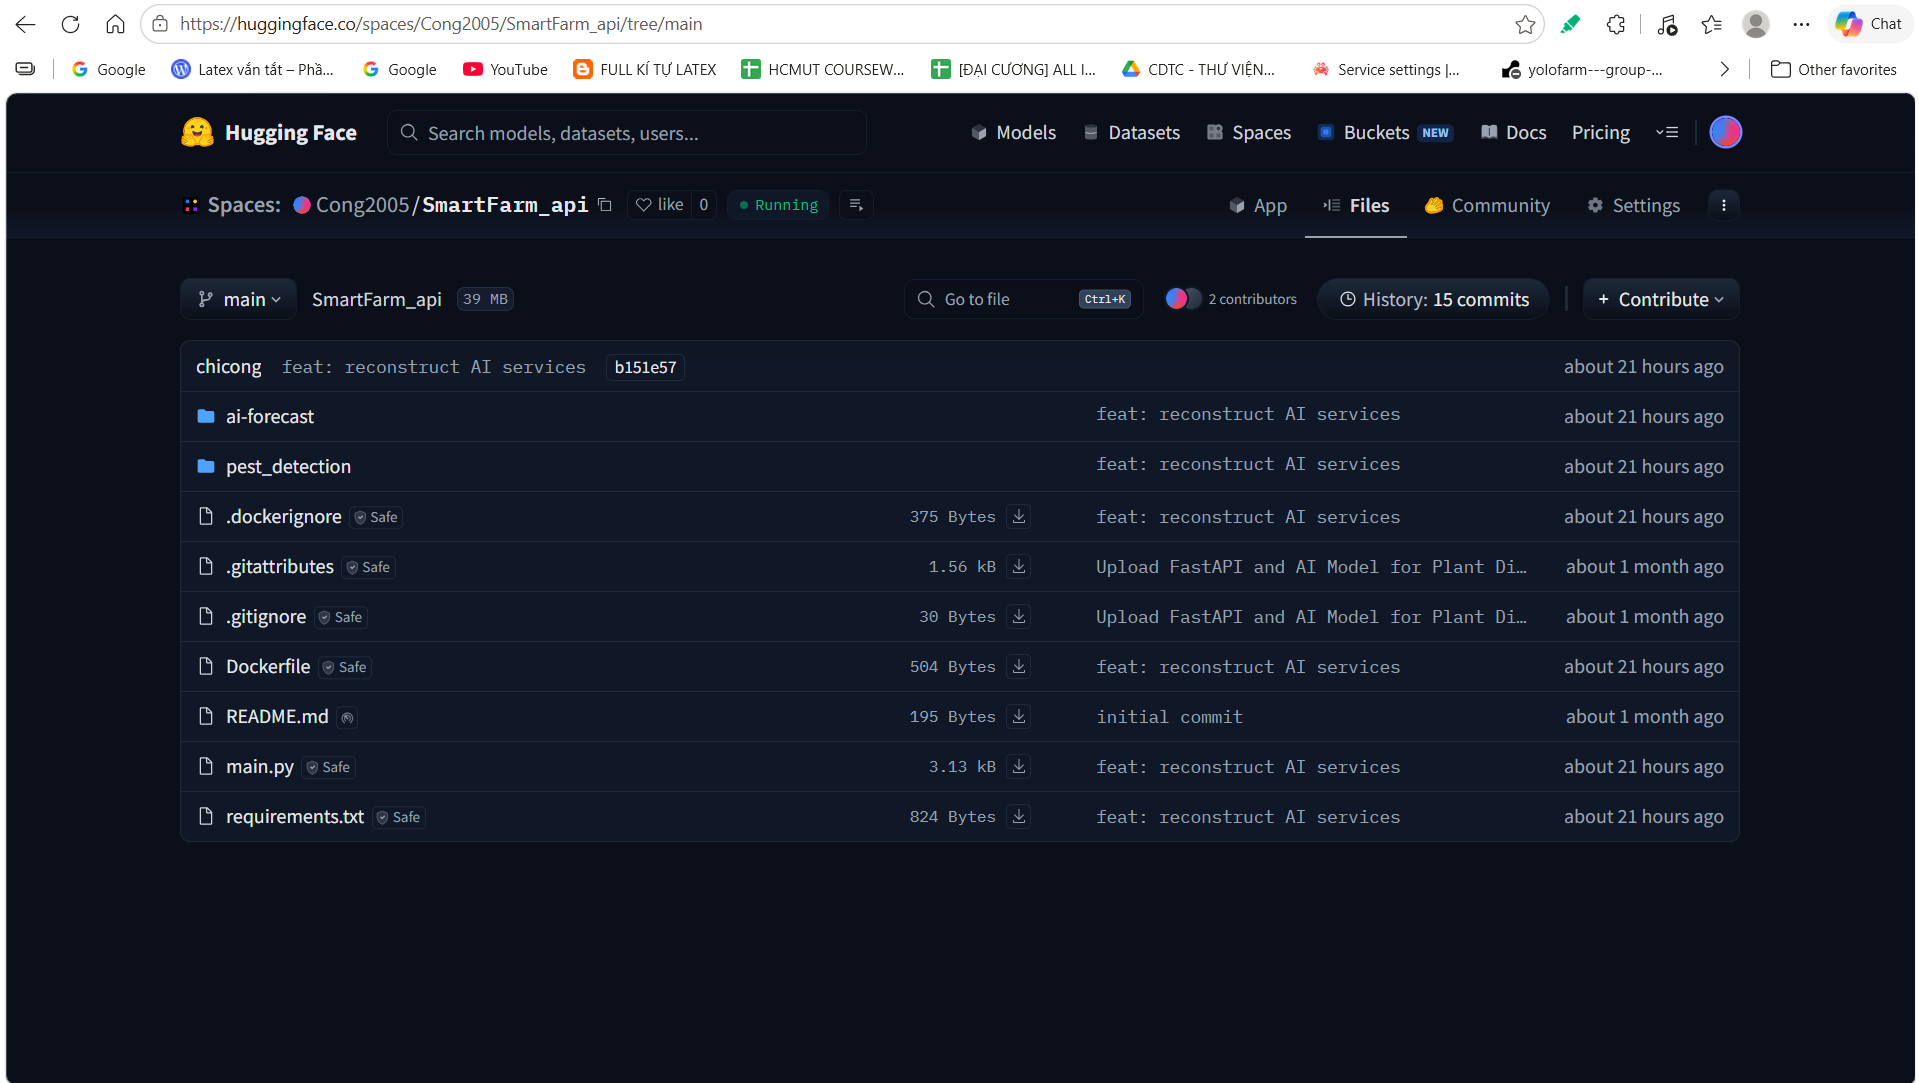
\includegraphics[width=0.8\linewidth]{./Pictures/Task_6/backend_AI_files.png}
	\caption{Hệ thống tự động biên dịch và chạy các mô hình AI}
\end{figure}
\subsubsection{Cơ chế hoạt động}
\indent Toàn thể kiến trúc YoloFarm được thiết kế theo hướng dễ mở rộng và tách biệt trách nhiệm:
\begin{itemize}
    \item \textbf{Luồng tương tác chính:} Người dùng làm việc trên frontend, frontend gửi request đến backend Node.js, backend xử lý nghiệp vụ và trả kết quả về giao diện. Cách tách lớp này giúp YoloFarm dễ bảo trì và phù hợp với cả chế độ chạy local lẫn triển khai container.
    \item \textbf{Luồng tải ảnh, chẩn đoán hoặc dự đoán độ ẩm:} Khi người dùng gửi ảnh lá cây để nhận diện bệnh, backend sẽ chuyển ảnh sang dịch vụ AI FastAPI độc lập, nhận kết quả dự đoán dạng JSON rồi phản hồi lại frontend để hiển thị cho người dùng. Mặt khác, khi bấm nút "Cập nhật dự báo" thì hệ thống dựa vào kho dữ liệu lưu trữ độ ẩm thực tế của ít nhất 24 giờ trước thời điểm cập nhật dự báo và dự đoán độ ẩm cho 24 giờ kế tiếp. Sau đó, kết quả dự đoán được trả về giao diện.
\end{itemize}